%! TEX root = main.tex

\graphicspath{{00_Images/05_chapter/}}

\chapter{Power in Audio Signals}
\label{ch:power}

Electrical power, mechanical power, and acoustic power are all described by the same mathematical structure: the product of two conjugate variables, one a pressure-like quantity and the other a flow-like quantity. In the electrical domain this is voltage times current; in the mechanical domain, force times velocity; in the acoustic domain, pressure times volume velocity. The challenge specific to audio engineering is that none of these signals is constant in time: musical waveforms are complex, non-periodic, and span many orders of magnitude in amplitude within a single piece. This chapter establishes the tools needed to quantify power in such signals, with particular attention to the distinction between mean and peak power and to the consequences for amplifier and transducer design.

\section{Electrical Power, RMS, and Crest Factor}
\label{sc:51}

The instantaneous electrical power delivered to a two-terminal element is:
\[
W_E(t) = v(t) i(t)
\]
For a purely resistive load \(R\), this becomes \(W_E(t) = v^2(t)/R\). Because audio signals have zero mean value by construction, the instantaneous power has a non-zero time-average even though the signal itself averages to zero. The physically relevant quantity is the mean power, defined as the time-average of the instantaneous power over a representative interval \(T\):
\[
\overline{W} = \frac{1}{T}\int_0^T W_E(t) dt = \frac{1}{R}\cdot\frac{1}{T}\int_0^T v^2(t) dt = \frac{v_\mathrm{RMS}^2}{R}
\]
where the Root Mean Square (RMS) voltage is:
\[
v_\mathrm{RMS} = \sqrt{\frac{1}{T}\int_0^T v^2(t) dt}
\]
The RMS value is the equivalent constant voltage that would dissipate the same energy in the resistance as the time-varying signal \(v(t)\). For a sinusoid \(v(t) = V_P\sin(\omega t)\), direct integration gives \(v_\mathrm{RMS} = V_P/\sqrt{2}\), which corresponds to a level 3 dB below the peak. The mean and peak power on a resistive load are then:
\[
\overline{W} = \frac{V_P^2}{2R}, \qquad W_\mathrm{peak} = \frac{V_P^2}{R} = 2 \overline{W}
\]

\paragraph{Musical signals in practice} Real musical waveforms are far more complex than a single sinusoid. The RMS value and the peak value both vary continuously as a function of the musical content, and the ratio between them changes from one moment to the next. The three intervals shown in the figure below illustrate how the same song can have very different peak-to-RMS ratios depending on the density and transient content of the passage.

\begin{figure}[!htb]
    \centering
    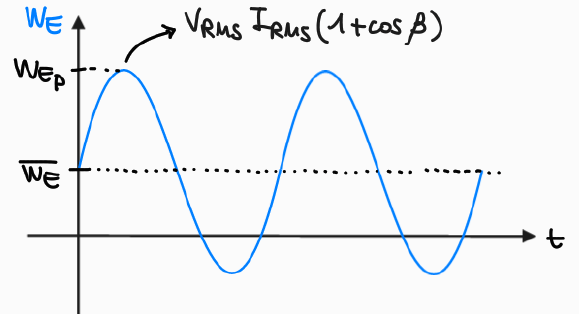
\includegraphics[width=0.85\textwidth]{electrical_power_wf.png}
    \caption{Three seconds of a typical musical signal divided into successive intervals. The RMS voltage (proportional to mean power) and the peak voltage vary independently across intervals, showing that both mean power and peak power are time-dependent quantities for audio signals}
\end{figure}

\subsection{The Crest Factor}
\label{ssc:511}

The ratio between peak power and mean power is called the Crest Factor (CF):
\begin{equation}
    CF = \frac{W_\mathrm{peak}}{\overline{W}}
    \label{eq:crestFactor}
\end{equation}
Expressed in decibels:
\[
CF_\mathrm{dB} = 10\log_{10}(CF)
\]
For a pure sinusoid, \(CF = 2\ (+\SI{3}{\decibel})\), because the peak power is exactly twice the mean power. For a complex musical signal, the crest factor is typically 4 or higher (\(\geq +6\) dB), and it depends on the time interval over which peak and mean values are measured: a transient-rich passage such as a percussion hit has a much higher crest factor than a sustained, compressed chord.
The crest factor has direct engineering implications. An amplifier must be capable of delivering the peak power without clipping, even if the mean power it supplies is much lower. If an amplifier is rated at a continuous output power \(\overline{W}\), and the musical signal has \(CF = 4\), then the amplifier must instantaneously supply \(4\overline{W}\) without distortion. Underestimating the crest factor leads to clipping on transients, which produces odd-order harmonic distortion and, more critically, can deliver sustained high-frequency content to a tweeter whose thermal rating is based on mean power: the voice coil overheats and the driver fails even though the rated mean power was never exceeded. Crest factor is therefore a key parameter for amplifier headroom specification and for loudspeaker thermal protection design.

\section{Power in a Generic Impedance}
\label{sc:52}

When the load is a complex impedance \(Z_E = R_E + jX_E\) rather than a pure resistance, voltage and current are no longer in phase, and the relationship between instantaneous and mean power requires a more careful treatment.
Consider a sinusoidal voltage \(v(t) = V\sin(\omega t)\) applied to an impedance \(Z_E\). The resulting current lags or leads the voltage by the phase angle \(\beta\):
\[
i(t) = I\sin(\omega t + \beta), \qquad I = \frac{V}{|Z_E|}
\]
The instantaneous power is:
\[
W_E(t) = v(t) i(t) = VI\sin(\omega t)\sin(\omega t + \beta)
\]
Expanding with the product-to-sum trigonometric identity:
\[
W_E(t) = \frac{VI}{2}\cos(\beta) - \frac{VI}{2}\cos(2\omega t + \beta)
\]
In RMS quantities (\(V_\mathrm{RMS} = V/\sqrt{2}\), \(I_\mathrm{RMS} = I/\sqrt{2}\)):
\[
W_E(t) = \underbrace{V_\mathrm{RMS} I_\mathrm{RMS}\cos(\beta)}_{\overline{W_E},\text{ constant}} - \underbrace{V_\mathrm{RMS} I_\mathrm{RMS}\cos(2\omega t + \beta)}_{\text{zero mean oscillation}}
\]
The time-average of the oscillating second term is zero over any complete cycle, so the mean power is:
\begin{equation}
    \overline{W_E} = V_\mathrm{RMS} I_\mathrm{RMS}\cos(\beta)
    \label{eq:meanPowerPhase}
\end{equation}

\subsection{In-Phase and Quadrature Decomposition}
\label{ssc:521}

The result of equation \eqref{eq:meanPowerPhase} can be made more transparent by decomposing the current into two components relative to the voltage. The in-phase component carries the portion of the current that is synchronized with the voltage:
\[
i_p(t) = I\cos\beta \sin(\omega t), \qquad i_q(t) = I\sin\beta \cos(\omega t)
\]
where \(i_p\) is exactly in phase with \(v(t)\) and \(i_q\) is 90 degrees out of phase (in quadrature). The instantaneous power separates accordingly:
\[
W_E(t) = v(t) i_p(t) + v(t) i_q(t) = W_{E,p}(t) + W_{E,q}(t)
\]
The active power component \(W_{E,p}(t) = V_\mathrm{RMS}I_{p,\mathrm{RMS}}[1 - \cos(2\omega t)]\) is always non-negative and has a positive mean equal to \(V_\mathrm{RMS}I_{p,\mathrm{RMS}}\): it represents energy flowing steadily from the source into the load, where it is converted into heat (in a resistance) or into mechanical or acoustic work. The reactive power component \(W_{E,q}(t) = V_\mathrm{RMS}I_{q,\mathrm{RMS}}\sin(2\omega t)\) oscillates symmetrically about zero and has a mean of exactly zero: it represents energy that is stored in the reactive element during one quarter-cycle and returned to the source during the next, with no net transfer per full cycle.
From the impedance relation \(i(t) = v(t)/Z_E\), one can extract the in-phase conductance:
\[
i_p(t) = \frac{\mathcal{R}\{Z_E\}}{|Z_E|^2} v(t)
\]
so the mean power is:
\[
\overline{W_E} = \frac{\mathcal{R}\{Z_E\}}{|Z_E|^2} V_\mathrm{RMS}^2
\]
Since \(I_\mathrm{RMS} = V_\mathrm{RMS}/|Z_E|\), this is equivalent to:
\begin{equation}
    \overline{W_E} = \mathcal{R}\{Z_E\} I_\mathrm{RMS}^2
    \label{eq:meanPowerZ}
\end{equation}
This result confirms that mean power is determined exclusively by the resistive (real) part of the impedance. The reactive part \(X_E\) shifts the phase between voltage and current, reduces the effective power factor \(\cos\beta\), and increases the current amplitude required to deliver a given mean power, but it contributes nothing to the time-averaged energy transfer.

\paragraph{Special cases} For a purely resistive load (\(X_E = 0\), \(\beta = 0\)): \(\overline{W_E} = V_\mathrm{RMS}^2/R_E\), the maximum possible power for a given voltage. For a purely reactive load (\(R_E = 0\), \(\beta = \pm\pi/2\)): \(\overline{W_E} = 0\), regardless of how large the instantaneous power swings become. A loudspeaker presents a complex impedance at almost all audio frequencies, so the power factor \(\cos\beta\) is always less than unity; this is why amplifiers must be rated for reactive loads and not merely for resistive ones.

\section{Mechanical and Acoustical Power}
\label{sc:53}

The same decomposition into active and reactive components applies in the mechanical and acoustic domains, with the appropriate substitution of power variable pairs.

\subsection{Mechanical Power}
\label{ssc:531}

The instantaneous mechanical power transmitted through a one-port mechanical element is \(W_M(t) = F(t) u(t)\). The mechanical impedance is defined as \(Z_M = F/u = R_M + jX_M\), where \(R_M\) is the mechanical resistance and \(X_M = \omega M_M - 1/(\omega C_M)\) is the reactive part. Under the admittance analogy, force maps to current and velocity maps to voltage, so the result of equation \eqref{eq:meanPowerZ} translates directly to:
\[
\overline{W_M} = R_M u_\mathrm{RMS}^2
\]
Only the resistive component of the mechanical impedance is responsible for net energy dissipation. In the loudspeaker, the total mechanical resistance has two contributions: the suspension damping \(R_{MS}\), which converts mechanical energy into heat within the spider and surround, and the mechanical radiation resistance \(R_{MR}\), which is the part of the mechanical load that transfers energy outward as acoustic radiation.

\begin{figure}[!htb]
    \centering
    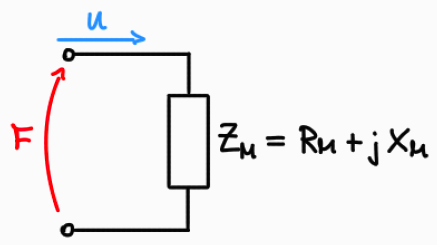
\includegraphics[width=0.35\textwidth]{mechanical_impedance_block.png}
    \caption{Mechanical one-port with impedance \(Z_M = R_M + jX_M\). The mean mechanical power is \(\overline{W}_M = R_M u_\mathrm{RMS}^2\); the reactive energy oscillates between mass and compliance without net loss}
\end{figure}

\subsection{Acoustical Power and the Radiation Resistance}
\label{ssc:532}

The instantaneous acoustic power is \(W_A(t) = P(t) U(t)\). The acoustic impedance is \(Z_A = P/U = R_A + jX_A\), and the mean radiated acoustic power is:
\[
\overline{W_A} = R_A U_\mathrm{RMS}^2 = \frac{\mathcal{R}\{Z_A\}}{|Z_A|^2} P_\mathrm{RMS}^2
\]

\begin{figure}[!htb]
    \centering
    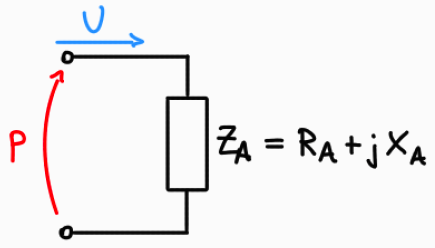
\includegraphics[width=0.40\textwidth]{acoustic_port_block.png}
    \caption{Acoustic one-port with impedance \(Z_A = R_A + jX_A\). Only \(R_A = \mathcal{R}\{Z_A\}\) contributes to net radiated acoustic power}
\end{figure}

For a loudspeaker, the acoustic radiation impedance at the diaphragm is \(Z_{AR} = R_{AR} + jX_{AR}\), where \(R_{AR}\) is the radiation resistance that converts diaphragm motion into propagating sound waves. Substituting the volume velocity \(U = u_c S_D\):
\[
\overline{W_A} = R_{AR} U_\mathrm{RMS}^2 = R_{AR} (u_c S_D)^2 = R_{MR} u_{c,\mathrm{RMS}}^2
\]
where the mechanical radiation resistance is:
\begin{equation}
    R_{MR} = S_D^2 R_{AR}
    \label{eq:mechanicalRadiation}
\end{equation}
Referred back through the electromechanical coupling \(F = Bl i_c\), and assuming that the coil inductance is negligible at the frequencies of interest (\(\omega L_{EC} \ll R_g + R_{EC}\)), the driving force is \(F_\mathrm{RMS} = Bl v_{g,\mathrm{RMS}}/(R_g + R_{EC})\), and the complete expression for radiated acoustic power as a function of generator voltage is:
\[
\overline{W_A} = \frac{R_{MR}}{|Z_M|^2} F_\mathrm{RMS}^2 = \frac{R_{MR}}{R_M^2 + X_M^2} (Bl)^2 \frac{v_{g,\mathrm{RMS}}^2}{(R_g + R_{EC})^2}
\]
This expression connects all physical parameters of the transduction chain to the single measurable quantity \(v_{g,\mathrm{RMS}}\) at the amplifier terminals.

\begin{figure}[!htb]
    \centering
    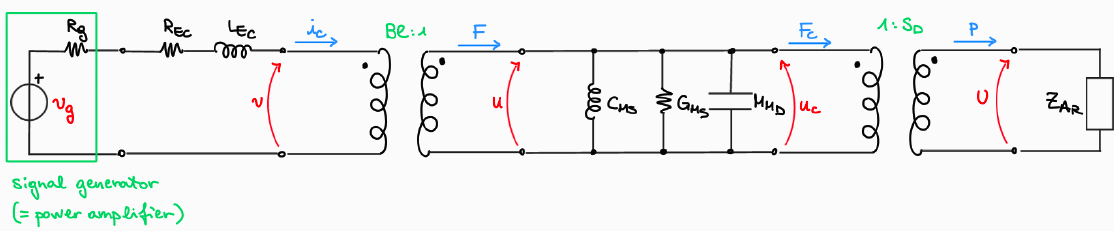
\includegraphics[width=0.75\textwidth]{electro_mech_acoustic_chain.png}
    \caption{Complete electrical-mechanical-acoustical chain of the loudspeaker. The power flow \(W_E \to W_M \to W_A\) is governed at each stage by the real part of the corresponding impedance; the reactive parts store and return energy without contributing to net radiation}
\end{figure}
